\begin{titlepage}
\begin{center}

% Upper part of the page. The '~' is needed because \\
% only works if a paragraph has started.

\includegraphics[width=0.35\textwidth]{figures/uom_banner.pdf}~\\[0.3cm]

\textsc{\Large Final Report}\\[0.3cm]

% Title
\HRule \\[0.3cm]
{ \huge \bfseries The Art of Scientific Computing:\\
Stereo Vision}\\[0.3cm]

\HRule \\[0.8cm]

% Author and supervisor
\begin{minipage}{0.45\textwidth}
\begin{flushleft} \large
\textit{Author:}\\
Haonan Li
\end{flushleft}
\end{minipage}
\begin{minipage}{0.45\textwidth}
\begin{flushright} \large
\textit{Subject Handbook code:}\\
COMP-90072
\end{flushright}
\end{minipage}
\\[1.0cm]

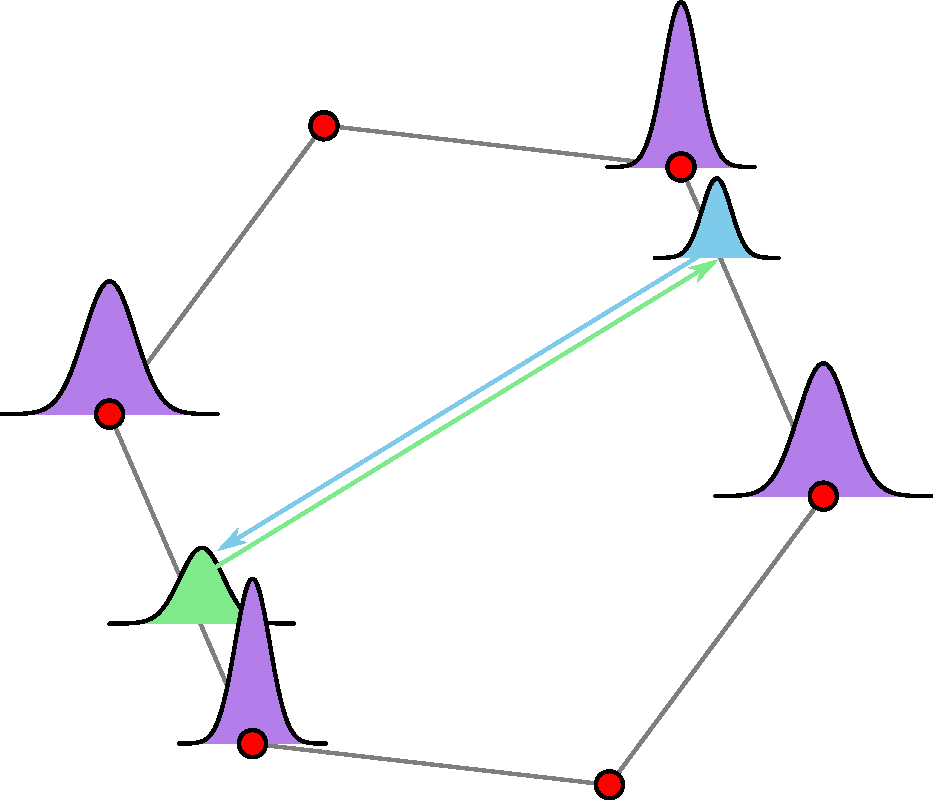
\includegraphics[width=0.50\textwidth]{figures/coulomb_direct.pdf}~\\[0.5cm]

\vspace{1.0cm}

% Place
The University of Melbourne
\\[0.5cm]

% Submission date
{\large 10 April 2018}
\\[1.5cm]

% Lecturer
Subject co-ordinators: A/Prof. Roger Rassool \& Kevin
\\[0.8cm]


% Bottom of the page
\end{center}
\end{titlepage}
